\documentclass{article}

\usepackage{amsmath}
\usepackage{amssymb}
\usepackage{tikz}
\usepackage[margin=2cm]{geometry}
\usepackage[super]{nth}
\usepackage{calc}
\usepackage{enumitem}
\usepackage{setspace}
\usepackage[utf8]{inputenc}

\usepackage[hidelinks, pagebackref, bookmarksopen, bookmarksnumbered]{hyperref}

\pgfdeclarelayer{bg}
\pgfsetlayers{bg,main}

\usepackage{esvect}

\usetikzlibrary{arrows,positioning,shapes,fit,calc}

\title{Mathematical Foundations for Software Engineering \\[1ex] \large Course notes}
\author{Attila Matolcsy}
\date{\nth{25} August 2023 - Present}

\let\stdsection\section
\renewcommand\section{\newpage\stdsection}

\usepackage[parfill]{parskip}

\begin{document}
\maketitle

\tableofcontents

\section{About}
This document is Attila Matolcsy's own personal notes from the University of Gothenburg's Software Engineering and Management Bsc. Programme's Mathematical Foundations for SEM course.

These are all the notes from lessons, unprocessed.

\begin{minipage}{\linewidth}
  \Large WARNING \vspace{.25cm}
\end{minipage}
This document has typos in it, please use the main document that is cleaned up!

\section{\nth{28} August 2023}

\subsection{Introduction to the course}

Lessons are not mandatory, nor the TA sessions.
We join a TA group on Canvas, we are asked not to jump between them. The gropus should not have more than 8 persons / group.

Workload $\approx 200 h$

Groups up to 3 are allowed but submissions must be on an individual basis.

FAQ is available on Canvas

You can send christian.berger@gu.se an email about problems that come up during class.

Course literature is available on Canvas, non of which is mandatory.

\subsection{Logic}

Logic = Meaning of mathematical statements $\wedge$ basis of reasoning

Applications = design of computing machines

$0$s $\And$ $1$s.

Proofs = matheatical argument, essential for programs \\ = Security of systems

Theorem = Proven mathematical statements

Propositions = declerative statemnt that is either True or False

For e.g.: \\
- Stockholm is the capital of Sweden \\
- $4x5 = 20$ \\
- $\pi \approx \frac{22}{7}$

Counter e.g.: \\
- attend my lectures \\
- $x + 1 = \pi$

Propositions are named by letters: $p, q, r, s$

field of propositional logic = the field that deals with propositionals

mathematical statements can be compined $\Rightarrow$ compoind propositions

Def1: $\neg p = $ not p

Def2: Conjuction: $p \and q$

\begin{tabular}{cc|c|c}
  $p$ & $q$ & $p \wedge q$  & $\neg \left( A \wedge B \right)$  \\ \hline
  $T$ & $T$ & $T$ & $F$ \\
  $F$ & $T$ & $F$ & $T$ \\
  $T$ & $F$ & $F$ & $T$ \\
  $F$ & $F$ & $F$ & $T$
\end{tabular}

(From now on I will refer to Trues ($T$s) as $1$ and Falses ($F$s) as $0$)

Def 3: $\vee$ is logical or\\
\begin{tabular}{cc|c}
  $p$ & $q$ & $p \vee q$ \\ \hline
  $1$ & $1$ & $1$ \\
  $1$ & $0$ & $1$ \\
  $0$ & $1$ & $1$ \\
  $0$ & $0$ & $0$
\end{tabular}

Def 4: exclusive or\\
\begin{tabular}{cc|c|c}
  $p$ & $q$ & $p \oplus q$ & $\neg \left( p \oplus q \right)$ \\ \hline
  $1$ & $1$ & $0$ & $1$ \\
  $1$ & $0$ & $1$ & $0$ \\
  $0$ & $1$ & $1$ & $0$ \\
  $0$ & $0$ & $0$ & $1$
\end{tabular}

Def 5: implication / conditional statements \\
\begin{tabular}{cc|c||c||c}
  $p$ & $q$ & $p \Rightarrow q$ & $\neg p \vee q$ & $\neg p$ \\ \hline
  $1$ & $1$ & $1$ & $1$ & $0$ \\
  $1$ & $0$ & $0$ & $0$ & $0$ \\
  $0$ & $1$ & $1$ & $1$ & $1$ \\
  $0$ & $0$ & $1$ & $1$ & $1$
\end{tabular}

Def 6: Biconditional statements, if and only if, iff\\
\begin{tabular}{cc|c}
  $p$ & $q$ & $p \Leftrightarrow q$ \\ \hline
  $1$ & $1$ & $1$ \\
  $1$ & $0$ & $0$ \\
  $0$ & $1$ & $0$ \\
  $0$ & $0$ & $1$
\end{tabular}

Def 7:
tantology: always true regardless of values of the propositions

Contardiction: always false regardless of values of the propositions

contingency: $\neg \left(\text{tantology}\right) \wedge \neg \left(\text{contradiction}\right)$

equivalents:\\
\begin{tabular}{ccc}
  $p \wedge 1$ & $\equiv$ & $p$ \\
  $p \vee 1$ & $\equiv$ & $1$ \\
  $p \wedge 0$ & $\equiv$ & $0$ \\
  $p \vee 0$ & $\equiv$ & $p$
\end{tabular}

$p \wedge q \equiv p$\\
\begin{tabular}{cc|c}
  $p$ & $q$ & $p \wedge q$ \\ \hline
  $1$ & $1$ & $1$ \\
  $0$ & $0$ & $0$ \\
\end{tabular}

negation laws:\\
$p \vee \neg p \equiv 1$ \\
\begin{tabular}{cc|c}
  $p$ & $\neg p$ & $p \vee \neg p$ \\ \hline
  $1$ & $0$ & $1$ \\
  $0$ & $1$ & $1$ \\
\end{tabular}

$p \wedge \neg p \equiv 0$ \\
\begin{tabular}{cc|c}
  $p$ & $\neg p$ & $p \wedge \neg p$ \\ \hline
  $1$ & $0$ & $0$ \\
  $0$ & $1$ & $0$ \\
\end{tabular}


\section{\nth{29} August 2023}

\subsection{Binary counting}

\begin{tabular}{|c|c|c|c|c|}
  \hline
  $\dots$ & $p$ & $q$ & $r$ & $s$ \\ \hline
  $x$ increases from right to left: $2^{x}$ & & & & \\
  This is what the binary number represents: & $2^3 = 8$ & $2^2 = 4$ & $2^1 = 2$ & $2^0 = 1$ \\ \hline
  This is our binary number: & $0 \left( F \right)$ & $1 \left( T \right)$ & $0 \left( F \right)$ & $1 \left( T \right)$ \\ \hline
  We need to sum this: $0 + 4 + 0 + 1 = 5$ & $0 \cdot 8 = 0$ & $1 \cdot 4 = 4$ & $0 \cdot 2 = 0$ & $1 \cdot 1 = 1$ \\ \hline
\end{tabular} \vspace{.5cm}


\subsection{Predicate Logic}

Propositional logic: everything is atomic

Predicate logic: Formalism of propositional logic is extended and more complicated expressions are possible to be ued for formal inference.

Predicate logic contains:

\begin{itemize}
  \item all components from propositional logic
  \item terms (E.g.: \underline{Alice} likes \underline{BOS} [Underlined is a term])
  \item quantifiers:
  \begin{itemize}
    \item something is always True
    \item something is sometimes True
    \item something is never True
  \end{itemize}
  \item Predicate symbols: $P, Q, R$
  \item functions: $f, g$
  \item quantifiers: $\forall, \exists$
  \item identity: $=$
\end{itemize}

Example: "There is a smallest number."

Collection of al persons, ideas, symbols, data structures that affect the logical argument under consideration

Elements of the inverese of the discourse are called individuals

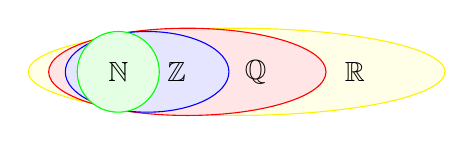
\begin{tikzpicture}
  \node (a) {$\mathbb{N}$};
  \node (b) [right = .25cm of a] {$\mathbb{Z}$};
  \node (c) [right = .5cm of b] {$\mathbb{Q}$};
  \node (d) [right = .75cm of c] {$\mathbb{R}$};
  \begin{pgfonlayer}{bg}
    \node[draw=yellow, fill=yellow!10, ellipse, fit = (a) (b) (c) (d)] (setD) { };
    \node[draw=red, fill=red!10, ellipse, fit = (a) (b) (c)] (setC) { };
    \node[draw=blue, fill=blue!10, ellipse, fit = (a) (b)] (setB) { };
    \node[draw=green, fill=green!10, ellipse, fit = (a)] (setA) { };
\end{pgfonlayer}
\end{tikzpicture}

\dots

Order of args is important

unary predicate: "x is a cat"
binary predicate: "y is mother of y"

unary predicates descripbe properties of object:
$ p \left( x \right) \Rightarrow $ x has property $ P $

interpret as: of a predicate ($P$) in a set of objects (called $A$) is a set og those elements of A (AKA subset) that have property p:

$ \left\{ \alpha \in A \quad | \quad P \left( \alpha \right)\right\} $

$ \left\{ (\alpha, \beta) \in A \times A \quad | \quad Q \left( \alpha, \beta \right)\right\} $


Atomic formula
\begin{enumerate}
  \item predicate name + arguments
  \item an identity $t_1 = t_2$
\end{enumerate}

Atomic formulas are statements that can be combined woth logical connectioves

$M \left( j, p \right) \rightarrow \neg M \left( p, j \right)$

If Jane is Paul's mother, then Paul is not Jame's mother.

If all arguments of a predicate are individual constants, the resulting formula must be \textcircled{T} or \textcircled{F}

Example:
\begin{tabular}{|c|cccc|}
  \hline
  & Bob & Jane & Alice & Paul \\ \hline
  Bob & F & F & F & F \\
  Jane & F & F & T & T \\
  Alice & F & F & F & F \\
  Paul & F & F & F & F \\
  \hline  
\end{tabular}

$M(a, b)$

Inly method that assigns truth values to all possible combinations of individuals is called assignment of the predicate



Universal quantifier: $\forall$

something is true for all infividuals

Existential quantifier: $\exists$

something is for at least one individual

\begin{tabular}{cl}
  $\forall \times A$ & $\forall$ = for all \\
  & $\times$ is bound by the quantifier \\
  & $A$ is the scope
\end{tabular}

Everone gets a break once in a while

$B(x) := $ "x gets a break in a while"\\
$\forall \times B\left(x\right)$

Some people don't eat meat

$p(x) := $ "x eats meat"\\
$\exists \times \left( \neg P \left( x \right)  \right)$

% Wait, are we still learning HS stuff?

$\exists x \left( \forall y k \left( x, y \right) \right)$

$\neg \exists x A\left( x \right) \equiv \forall x \neg A$

\end{document}